%=========================================================================
% (c) Michal Bidlo, Bohuslav Křena, 2008

% Zajimavy blog
% http://brendangregg.com/

\chapter{Introduction}
\label{Introduction}
Good application performance is one of the main goals during the software development. But what makes software performance so important? Poor performance can have very unpleasant behavior not just for its users, but also for the application owners. Software reliability is guaranteed by the owner, but with undesirable performance there could be a lot of issues which can badly influence software behavior. And this can lead to a significant outflow of the consumers, and even brand destruction, financial damage or loss of trust. These few reasons should be enough to do a proper performance testing before software release, especially for many of large projects where industries guarantee certain level of software behavior and they cannot assure it after insufficient performance testing. Great emphasis on software performance is in particular in space programs, medical facilities, army systems or energy distribution systems. In such cases it is necessary to ensure proper application behavior for a long time under high load and without unsuspected behavior such as high response time, frequent delays or timeouts, because every failure could cost a lot of money. 

Nowadays every developer should try to use well established \todo{Doplnit vyznam well estabilished} frameworks which can make developers work easier because they handle complex underlying issues such as security, performance and code clarity. This way developers can invest more time in the application functionality and meet the application requirements, since frameworks are usually optimized for one particular job. In the past every developer had to spent more time tuning performance which lead to spending more time and money for software development. But not everyone has enough knowledge about performance testing and this makes performance analysis and optimization even more difficult. This leads to a need to specialized performance tools which can provide more sophisticated information. However, useful tools are usually proprietary or expensive.

A very important part of the performance analysis is the right choice of \emph{key performance indicators} (KPIs) \cite{Molyneaux:TAoAPT} and effective interpretation of the results. This can lead to faster detection of performance problems and help developers to fix them and meet the \emph{performance standards} \cite{Molyneaux:TAoAPT} set up by application owner or customer in time before the release. 

In general an application performance is very important however nowadays smooth network application or hardware performance became much more demanded nowadays since most of the communication is via the internet.  Obviously when you make payment in your internet banking you definitely want to have a stable connection to your bank's website without any delay. Network components like routers and switches influence the network stability, hence it is very important to care about performance of those components. Network performance testing refers to measures of service quality of a network which is directly influenced by \emph{bandwidth, throughput, latency}, etc. 

For performance testing of network messaging system developed by \emph{Red Hat Inc.} there is existing solution\,---Messaging Performance Tool (MPT) \cite{ORPISKE:MSGPT}. MPT is specialized for performance testing of \emph{Broker tool} \cite{RH:Broker}\,---\,network application level software cooperating with \emph{Qpid-dispatch tool} \cite{RH:Interconnect} in the network as the message distributor. Unfortunately, current version of MPT does support performance testing of the Router component, Qpid-dispatch. 

This thesis is structured as follows. First, define fundamentals of performance testing Chapter \ref{Fundamentals of Software Performance Testing}. The rest of thesis is focuses on performance testing and analysis of Qpid-dispatch, an application level router designed by Red Hat Inc. Qpid-dispatch performance testing is based on MPT described in Chapter \ref{Messaging Performance Tool}. Description includes \emph{measures process} and \emph{gathered data description and evaluation}. Main goal is to analyze MPT and design module for Qpid-dispatch performance testing. This part can be found in Chapter \ref{Analysis and Design} together with protocols which router uses and \emph{Automatic Topology Generator} for semi-automated network generating and deployment. After appropriate design, the implementation is needed, all used technologies, tools and  implementation processes of each component are described in Chapter \ref{Implementation}. The most important part of the thesis is in Chapter \ref{Experimental Evaluation}. It contains gathering data from routers located in different types of topology, their evaluation and representation which leads to conclusion about performance of Qpid-dispatch. Finally, Chapter \ref{Conclusion} summarizes the thesis and proposes ideas for future use of developed tool.

% https://www.seguetech.com/what-is-software-performance-testing/

\chapter{Fundamentals of Software Performance Testing}
\label{Fundamentals of Software Performance Testing}
Usual goal of performance testing is to ensure that the application runs reasonably fast enough to keep the attention of users, even with unexpected number of users using the application at the same time. Why is it so important to have application optimized for best speed? It is simply, when your application have slow response, long load time or bad scalability, the first website which user visit afterwards will be web of your competitor. That is the reason why speed is one of the most significant performance factor of common performance problems. This chapter summarizes fundamentals of performance testing which includes common performance processes, issues and metrics. This chapter is based on knowledge available in \cite{Molyneaux:TAoAPT, Kurkova:Thesis:2017, DIN:PHD}.


\section{Performance Testing Process}
\label{Performance Testing Process}
The main goal of performance testing is to ensure the following application attributes \cite{GAO:MEASURING}:

\begin{itemize}
	\setlength\itemsep{0em}
	\item \textbf{Reliability and Stability}\,---\,the ability of software to perform its functions in system environment under some system load for acceptable period of time,
	\item \textbf{Scalability}\,---\,the ability of software to behave properly under various types of system load and handle growing up amount of workload (network traffic, server load, data transfer, etc.),
	\item \textbf{Processing time, Speed}\,---\,the ability of software to react quickly without low response time during any acceptable system load,
	\item \textbf{Availability}\,---\,the ability of software to make all of its functions available during any acceptable system load.
\end{itemize}

Performance testing process, similarly to software development process, consist of all engineering steps ranging from requirements definition to data evaluation. These steps also includes design, implementation of performance tests and execution with data gathering. Graphical representation of the performance testing process is depicted in the Figure~\ref{fig:performace_testing_process}. 

\begin{figure}[H]
  \centering
  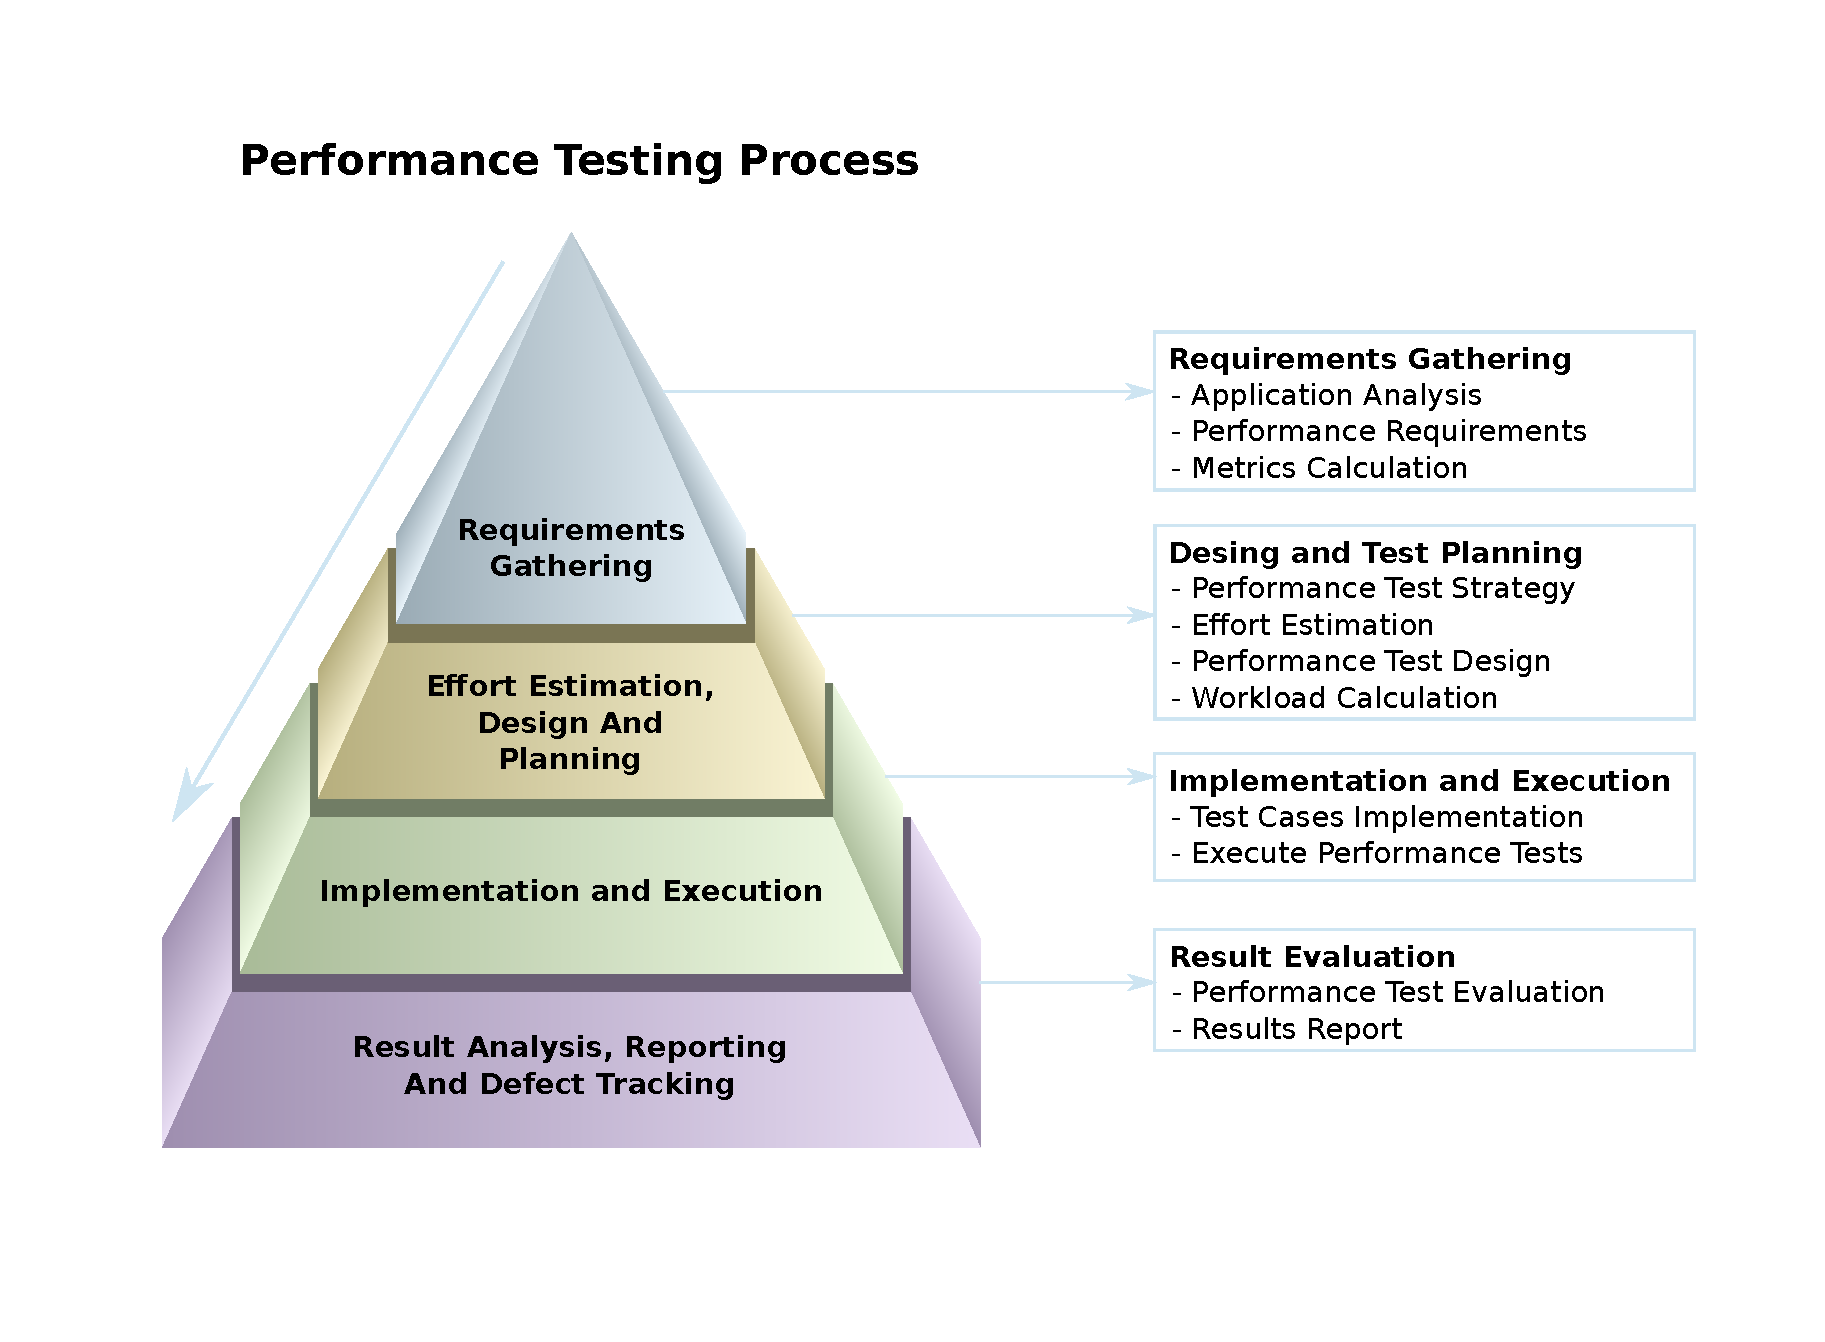
\includegraphics[width=16cm]{obrazky-figures/pyramid.pdf}
  \caption{Pyramid scheme of Performance Testing Process \todo{vice popsat}}
  \label{fig:performace_testing_process}
\end{figure}

The first step of performance testing process is the selection of \emph{performance requirements} for the application. In this step, testing engineer has to analyze tested application, describe performance metrics, which will model the application performance and set performance requirements. The result should include answers such as:

\begin{itemize}
	\setlength\itemsep{0em}
	\item How many end users will the application need to handle at release, after 6 months or in 1 year ?
	\item Where will these users be physically located, and how will they connect to the application?
	\item How many end users will be concurrently connected in average at release, after 6 months and 1 year?
\end{itemize}

Based on answer to these studies, the engineer should be able to select important key performance indicators for performance test cases. Some of these indicators may be eg. \emph{response time}, \emph{stability}, \emph{scalability} and \emph{speed}. However there is huge number of possible indicators so it is necessary to analyze whole application and also take into consideration another needs like an error rate, system resources etc.  Result of this phase should be a binding document with all performance requirements to be tested and, in case of detected performance degradation, this defect must be fixed according this document.

The next step is to define the \emph{performance testing strategy}, corresponding to planning and design. It is extremely important to allocate enough time for test application effectively, because, as it was mentioned in Chapter \ref{Introduction}, performance testing is not an easy task and detecting all of the possible issues of tested units is very time consuming process. Every plan should take into account the following considerations:

\begin{itemize}
	\setlength\itemsep{0em}
	\item \textbf{Prepare test environment}\,---\,proper environment needs sourcing and configuring proper hardware\todo{preformulovat}.
	\item \textbf{Provide sufficient workload injectors}\,---\,prepare workload injector may take few days; this usually involves a few workstations or servers to simulate real traffic.
	\item \textbf{Identify and script use cases}\,---\,this include identification of important parts of system which may have an impact on performance; time needed for each use case may be different because some use cases can be simple such as navigating to a web application home page or complex such as filtering specific communication
	\item \textbf{Performance test scenario}\,---\,\todo{doplnit}.
	\item \textbf{Instrument the test environment}\,---\,install and configure the monitoring software on the test environment.
	\item \textbf{Deal with detected problems}\,---\,test can detect significant performance issues and their fix may take a long time.
\end{itemize}

While this process seems trivial, the opposite is true, in particular in case of network applications. Most of performance issues manifest any big workload or high number of users, eg. when million users are sending requests to the network device at the same time it could lead to unacceptable device crash. Workload injectors are designated to simulate real user activity, and allows automatic analysis of performance behavior for tested application or device. Depending on the used technology, there can be a limit on the number of virtual users that can be generated by a single injector. Automated workload injectors are necessary for effective performance testing.

After determining the plan we implement and execute designed test cases. Environment and workload injectors are ready for execution, so last thing before testing itself is the implementation of tests. Thanks to the previous step, engineers should have enough time to implement designed test cases precisely as they were designed. 

Final step of performance testing process is results evaluation. Output of this step is usually technical report with all selected performance key indicators, used workload and gathered data for each test cases. Then follows the data evaluation with thorough analysis of degradation tracking. Additionally, the report also contains syntactical graphs which display performance metrics along the duration of test execution.

\section{Performance Issues}
\label{Performance Issues}
Performance issue is a common label for an unexpected application or device behavior which affects its performance. Usually, those issues are hard to detect because they manifest only under certain circumstances such as high load or long application run time. In the network applications there are several issues that are more frequently occurring  than others. In following, we will describe chosen issues in more detail.

\subsection{Performance Degradation}
Unclean code usually leads to inefficient algorithms, application deadlocks or memory leaks, which all can eventually lead to performance degradation. The problem is that these issues are usually detected only during the long run time of application or inability of an application to handle high load. For this kind of issues there is a performance testing method called \emph{soak testing} \cite{BUCH:4TYPES, Manzor:APTB} which is described in Section \ref{Soak Testing}. In short term, soak test is intended to identify problems that may appear only after long period of application run time, hence its necessary to run this type of tests during network application development since they usually need to be available for 24 hours per day. The duration of a soak test should have some correlation to the operational mode of the system under test. Following scenarios may contains performance issues detectable by soak tests:

\begin{itemize}
	\setlength\itemsep{0em}
	\item a constant degradation in response time, when the system is run over time,
	\item any degradation in system resources that are not apparent during short runs but will surface during long run time such as free disk space, memory consumption or machines handles,
	\item a periodical process that may affect the performance of the system, but can be detected only during long run time as backup process, exporting of data to a 3rd party system, etc.
\end{itemize}


\subsection{Response Time}
Response time is time it takes system to accept, evaluate and response to the user for his request . Different actions and requests can have significantly different response time and with that provide different load on the system. For example retrieving document from web-server by its ID is considerably faster than searching for the same document by keywords. Response time is measured during \emph{load test} \cite{Manzor:APTB} of the application. Well designed test should consider different type of load on the system, which means various kind of requests, and different 
number of connected end-users at the same time. usually we put 3 limits for the response time values: 

\begin{itemize}
	\setlength\itemsep{0em}
	\item \textbf{0.1 second}\,---\,this represent an ideal response time for the application, because user feels that system is reacting instantaneously and does not sense any interruptions,
	\item \textbf{1 second}\,---\,this is the highest acceptable response time when user still does not feel any interruptions, but user can feel a little delay; so far no bad impact on user experience,
	\item \textbf{10 second}\,---\,this is the limit after which response time become unacceptable and user will probably stop using your application.
\end{itemize}

\todo{First iteration till here!}

\subsection{Traffic Spikes}
As \emph{traffic spikes} \cite{Kurkova:Thesis:2017, AMC:SPIKES} we can understand the sudden degradation of one of the performance metrics such as \emph{throughput, bandwidth, error rate, response time} but also recourse usage such as \emph{memory usage, disk space, etc.} In real network, spikes are result of high workload, which can be caused by multiple users trying to concurrently use service over the network. For example after publishing new popular viral context on video servers, start of sales events, reservation of limited count of tickets or subject registration at university.

Traffic spikes can lead to inappropriate system behavior such as \underline{long response time}, \underline{bad throughput} and \underline{limited concurrency}. For prevent influence of traffic spikes on system performance, it's  necessary to do sophistic infrastructure monitoring and network load analysis, because we should recognize normal traffic and attack on the system. Method designed for spikes testing is called \emph{stress testing} \cite{Manzor:APTB} and it's described in Section \ref{Different Types of Performance Testing} in detail. Network system should also be scalable, thus it should be able to redirect traffic to another node with same service in case of high load which can cause performance issues due inappropriate recourse usage.

\begin{figure}[H]
  \centering
  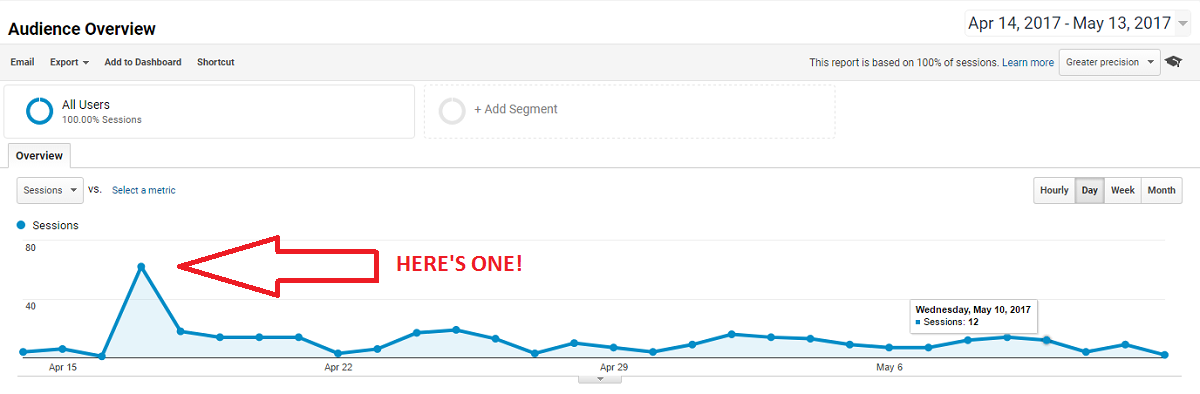
\includegraphics[width=15cm]{obrazky-figures/spike.png}
  \caption{\todo{Najit novy}}
  \label{fig:spikes}
\end{figure}

In the Figure \ref{fig:spikes} there is recorder traffic spike of.....\todo{popsat obrazek}

\section{Different Types of Performance Testing}
\label{Different Types of Performance Testing}
% % http://www.wmrichards.com/high_performance_messaging.pdf 2017/10/18

For performance measurements there are many types of tests. Which test you should use is determined by nature of the system, testing requirements and how much time is available for performance testing. The following testing term are generally well known and using in practice and each of them characterizes category or suite of the tests. The following subsections are based on knowledge available in \cite{TuPo:TESTS, BUCH:4TYPES, Molyneaux:TAoAPT}.

\subsection*{Load Testing}
Load testing is a testing method which examines how developed system behaves during different types of workload within its acceptable limits. Basically its simulation of real-world load. Main metric to focus during load test is response time of the system on requests from users or another system which communicating with tested subject. Main goal is to determine if system can handle required workload from performance requirements. Load tests are designed to measure response time of system transactions under normal or peak workload. When the systems response time dramatically extends or become unstable, thus system reach its maximum operating capacity. After this, engineers will mark workload requirements as fulfilling or they should analyze gathered data and report issues to the developers. In the Figure \ref{fig:load_test} you can see graph of load test showing workload of 1.000 users who are sending requests to the web server at the same time where the system response time does not exceed 2 seconds.

\begin{figure}[H]
  \centering
  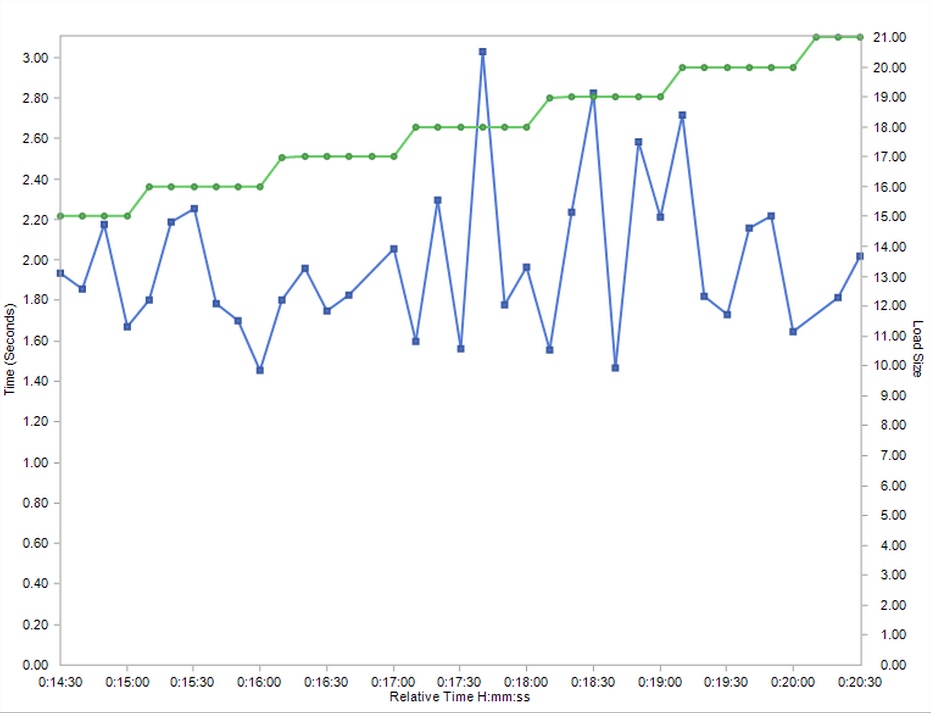
\includegraphics[width=15cm]{obrazky-figures/load-testing.png}
  \caption{\todo{vlastni obrazek - popsat}}
  \label{fig:load_test}
\end{figure}

\subsection*{Stress Testing}
\label{Stress Testing}
Stress testing is the specific type of load test, where engineers does not measure normal workload, but focus on unexpected workloads and traffic spikes. The main purpose is to find how the system behaves in extreme conditions such as enormous number of concurrent requests, using a server with much less memory or a weaker CPU and analyze system performance threshold. Its very useful to know performance threshold because you want to know the difference between performance under normal workload and performance threshold when the system is overloaded. The following enumeration collect common stress test scenarios: 

\begin{itemize}
	\setlength\itemsep{0em}
	\item Monitor the system behavior when maximum number of users logged in at the same time,
	\item All user performing critical operations at the same time,
	\item All users accessing the same file at the same time,
	\item Hardware issues such as server in cluster down.
\end{itemize} 

When engineers finish stress testing and found systems limits, they also can test the system recovery after crash during finding of the system limits.

\begin{figure}[H]
  \centering
  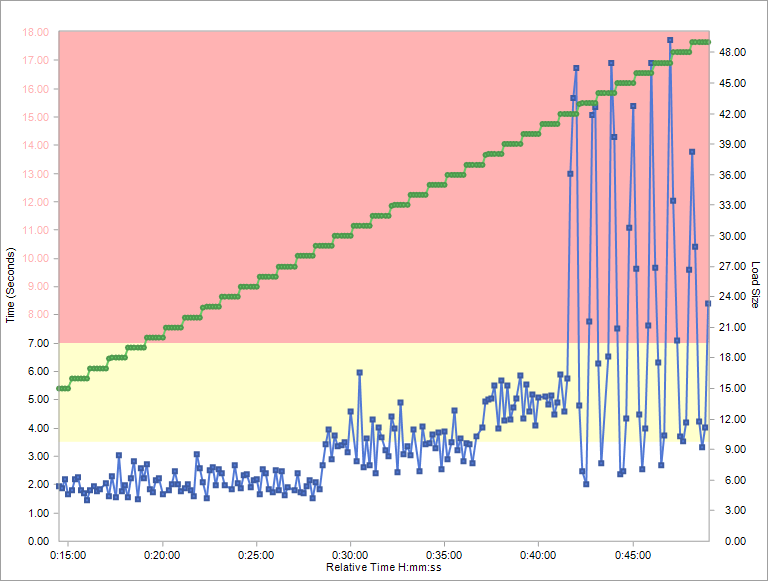
\includegraphics[width=15cm]{obrazky-figures/stress-testing.png}
  \caption{\todo{vlastni obrazek - popsat}}
  \label{fig:load_test}
\end{figure}

\subsection*{Soak Testing}
\label{Soak Testing}
Soak, or stability/endurance testing refer to method, where goal is to identify problems, that may appear only after extended period of time. The system seems stable for one week, but after longer period than that, problems such as memory leaks or not enough disk space can appear. Primary measured metric during soak tests is memory. The following are common issues found by soak test:

\begin{itemize}
	\setlength\itemsep{0em}
	\item Serious memory leaks that will eventually result into system crash,
	\item Improperly closed database connections could starve the system,
	\item Improperly closed connections between system layers could stall any of the system modules,
	\item Step-wise degradation could lead to high response time and the system become inefficient.
\end{itemize}

This sort of test needs for effectively use appropriate monitoring system. Problems detected by soak tests are typically manifested by gradual system slowdown in response time or as sudden lost of system availability.

\begin{figure}[H]
  \centering
  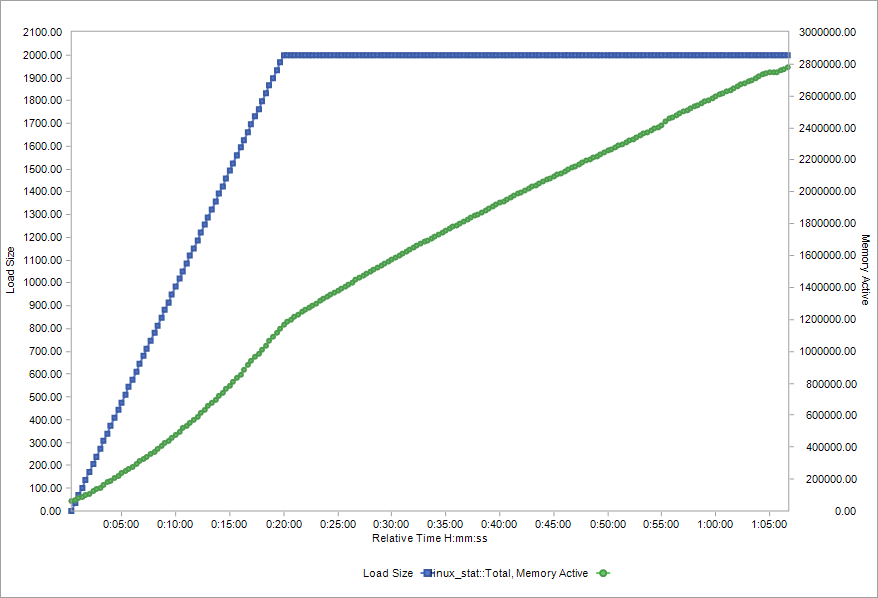
\includegraphics[width=15cm]{obrazky-figures/soak-testing.png}
  \caption{\todo{vlastni obrazek - popsat}}
  \label{fig:load_test}
\end{figure}

\subsection*{Smoke Testing}
Smoke testing method is inspired by similar hardware technique, when engineers checks for the smoke from the device after tuning power on. Basically, its very similar for software, since main goal of smoke test is to test basic functionality of the system and tell to the engineers if the system is ready for build. However, smoke tests are testing functionality on a surface level, so its not enough for testing deeply basic systems functions. When smoke tests fails, the system are tagged as unstable, because its can't ensure basic functionality and its not tested anymore until the smoke test will pass because it should be waste of time. Smoke test are designed to uncovering obvious errors which saves time, money and effort of the engineers. Smoke tests should be used with every new build, since new features could harm previous system functionality. 


\subsection*{Regression Testing}
With software development comes times, when engineers develop new feature and they want to update previous build and now is the time for regression testing. \emph{Regression tests} \cite{STF:REGRESSION} are designed to test functionality of the latest build updated with new feature. The main objective is to determine, if new feature affects already functional parts of the system. This type of tests are very important, because engineers do not always know, which part of the system will be indirectly affected. During regression testing, new test cases are not created, but previous test cases are automatic re-executed and analyzed. 


\subsection*{Benchmark Testing}
\emph{Benchmark testing} \cite{Aho:Benchmarking} is method, which is collecting performance data during the system run on different hardware machines. Gathered data have significant value when we want smooth run of the system on an older hardware, hence we can discover performance issues under normal load. However, the system does not run smoothly on prepared hardware, only options is to run benchmark tests on different machines with different hardware and under different load. \todo{dopsat nebo vyhodit} 

\section{Performance Metrics}
\label{Performance Metrics}
% https://loadstorm.com/load-testing-metrics/ 2017/10/18

\subsection{Response Time}

\subsection{Requests per Second}

\subsection{Resource Usage}

\subsection{Throughput}

\subsection{Error Rate}

\chapter{Messaging Performance Tool}
\label{Messaging Performance Tool}
% https://github.com/orpiske/msg-perf-tool

\section{Measures Process}
\label{Measures Process}

\section{Testing Metrics}
\label{Testing Metrics}

\section{Gathered Data and Their Evaluation}
\label{Gathered Data and Their Evaluation}

\section{Related Works}
\label{Related Works}
% popsat podobne "existujici" reseni (samozrejme, obcas neexistuje ;), ale verim, ze zde se neco najde). Nejlepsi je i se vuci tem "related tools" vymezit (jako napr. "The tool ... cannot be used because it does not support ...")

SpecJMS

\chapter{Analysis and Design}
\label{Analysis and Design}

\section{Qpid-Dispatch Router}

\section{Usable Protocols}
AMQP, MQTT - possibly?

\section{Automatic Topology Generator}

\subsection{Network Components}

\subsection{Structure of Input and Output}

\subsection{Topology Creation}

\section{Qpid-Dispatch Performance Module}

\subsection{TODO - more subsections about module}

\section{Performance and Testing Metrics of Qpid-Dispatch Performance Module}

\section{Gathered Data Evaluation}

\chapter{Implementation}
\label{Implementation}

\section{Used Technologies}

\subsection{Ansible}

\subsection{Docker}
Using for testing Ansible roles (remove?)

\section{Topology Generator}

\subsection{Template Generator}

\subsection{Generation of Variables}

\subsection{Configuration Files Generation and Deployment}

\section{Qpid-Dispatch Performance Module}

\subsection{TODO - more subsections about implementation}

\chapter{Experimental Evaluation}
\label{Experimental Evaluation}

\section{Performance Testing on Various Generated Topology}

\section{Testing results}

\chapter{Conclusion}
\label{Conclusion}
%=========================================================================
